\documentclass[10pt, letterpaper]{article}

\usepackage[margin=1in]{geometry}
\usepackage[T1]{fontenc}
\usepackage{lmodern}
\usepackage{amsmath, amssymb, amsthm}
\usepackage{booktabs}
\usepackage{graphicx}
\usepackage{xcolor}
\usepackage[hidelinks]{hyperref}
\usepackage{enumitem}
\usepackage{caption, subcaption}
\usepackage{listings}

\lstdefinelanguage{lean}{
  keywords={theorem, lemma, def, inductive, structure, where, fun, match, with,
            namespace, end, import, deriving, let, have, obtain, exact, intro, rintro},
  sensitive=true,
  comment=[s]{/-}{-/},
  morecomment=[l]{--},
}
\lstset{
  language=lean,
  basicstyle=\small\ttfamily,
  keywordstyle=\bfseries,
  commentstyle=\itshape,
  columns=fullflexible,
  keepspaces=true,
  breaklines=true,
  xleftmargin=1.5em,
}

% Allow modest interword stretch as a last resort so long typewriter
% Lean identifiers do not produce overfull lines (render-gate hygiene).
\emergencystretch=3em

\newtheorem{theorem}{Theorem}[section]
\newtheorem{lemma}[theorem]{Lemma}
\newtheorem{definition}[theorem]{Definition}
\newtheorem{corollary}[theorem]{Corollary}
\theoremstyle{remark}
\newtheorem{remark}[theorem]{Remark}

\newcommand{\lean}[1]{\texttt{#1}}
\newcommand{\TLP}[1]{TLP~#1}

\title{Independence as a Modeling Choice:\\
  The Geometry of Tractarian World Models}
\author{Robb Walters}
\date{July 2026}

\begin{document}
\maketitle

\begin{abstract}
The \emph{Tractatus} asserts that states of affairs are mutually independent
(\TLP{1.21}, \TLP{2.061--2.062}); the color-exclusion problem (\TLP{6.3751};
Wittgenstein 1929) is standardly told as this thesis's refutation and the
proximate cause of the book's collapse. We retell the story
model-theoretically, on a machine-checked foundation. Rather than asking
whether independence is \emph{true}, we treat it as a \emph{modeling choice}:
the free model is a distinguished point in a space of world models ordered by
a refinement preorder, whose structure we develop --- evaluation is preserved
along refinements, tautologies and contradictions are inherited downward, the
free model is the maximum and is unique up to refinement-isomorphism among
models realizing every truth-value profile, and refinement is a lattice-like
order captured exactly by image-profile sets, with joins, meets, and
infinitary joins. Constraint classes carve this space into tiers. For Horn
constraints (positive implications between states of affairs) we state an
exact realizability boundary that renders \TLP{2.061} precise. Our central
new result concerns \emph{exclusion} constraints
$\neg(a \wedge b)$ --- the formal shape of color exclusion: no Horn constraint
set is refinement-equivalent to any nontrivial exclusion model. Wittgenstein's
1929 crisis thus becomes a separation theorem about the geometry of logical
space. All results are formalized in Lean~4 and checked by its kernel: 64
declarations, no \lean{sorry}s, axiom footprint limited to propositional
extensionality, choice, and quotient soundness.
\end{abstract}

\section{Introduction}\label{sec:intro}

The \emph{Tractatus Logico-Philosophicus} builds its account of logic and
representation on a striking structural postulate: the mutual independence of
states of affairs.
\begin{quote}
  1.21\quad Each item can be the case or not the case while everything else
  remains the same.\\[2pt]
  2.062\quad From the existence or non-existence of one state of affairs it is
  impossible to infer the existence or non-existence of another.
  \cite{wittgenstein1921}
\end{quote}
Independence is what makes the truth-table picture of propositions work:
if $n$ states of affairs can obtain or fail in any combination, logical space
has exactly $2^n$ points, every elementary proposition is logically neutral
with respect to every other (\TLP{4.211}), and all necessity is truth-functional
necessity.

The standard narrative is that this postulate destroyed the book. Ramsey's
review already pressed the problem of color ascriptions
\cite{ramsey1923}; Wittgenstein himself flagged the case in \TLP{6.3751} ---
``the simultaneous presence of two colours at the same place in the visual
field is \ldots ruled out by the logical structure of colour'' --- and in
``Some Remarks on Logical Form'' finally conceded that attributions of degree
exclude one another in a way his truth-functional apparatus cannot represent
\cite{wittgenstein1929}. Hacker's verdict is representative: on his
telling, Wittgenstein's first philosophy collapsed over its inability to
solve this one problem --- colour exclusion \cite{hacker1986}.

This paper retells the story in a different register. We do not ask whether
the independence thesis is true, nor whether some choice of elementary
propositions rescues it (that is Moss's project \cite{moss2012}, engaged in
\S\ref{sec:discussion}). We treat independence as a \emph{modeling choice}: one
admissible answer --- the maximally permissive one --- to the question of which
truth-value profiles over the states of affairs are realized by some possible
world. Under this reframing the interesting object is not the thesis but the
\emph{space of alternatives to it}: the collection of world models, ordered by
how much independence they retain, with the fully independent \emph{free
model} at the top. The color-exclusion problem then stops being an
embarrassment to be explained away and becomes a structural datum: the
constraint that broke the book lives in a provably different region of this
space than the constraints the book's machinery can absorb.

Concretely, we develop the following picture (Figure~\ref{fig:spectrum}). A
\emph{world model} over a type $S$ of states of affairs is a nonempty family
of worlds together with a relation saying which states obtain at which world;
its \emph{image profiles} are the truth-value patterns over $S$ it realizes.
A \emph{refinement} $M \sqsubseteq M'$ is a profile-preserving map from
$M$-worlds to $M'$-worlds: passing down the order adds constraints, passing up
removes them. Within this order:

\begin{enumerate}[label=(C\arabic*), leftmargin=3em]
\item\label{c:spectrum} \textbf{The spectrum.} Refinement is a preorder with
  the free model as maximum; evaluation of propositions is preserved along
  refinements, so tautologies and contradictions propagate from freer to more
  constrained models; and a proposition holds at \emph{every} model of the
  spectrum iff it is a tautology of the free model. Logical truths are
  exactly the propositions insensitive to the modeling choice
  (\S\ref{sec:spectrum}).
\item\label{c:unique} \textbf{Uniqueness of the free model.} Among models
  realizing every profile, the free model is unique up to
  refinement-isomorphism: full independence pins the model down
  (\S\ref{sec:spectrum}).
\item\label{c:lattice} \textbf{The lattice of logical space.} Refinement
  between models is equivalent to inclusion of image-profile sets, and the
  order carries joins, meets, and infinitary joins computed exactly by unions
  and intersections of image profiles. The ``geometry'' of Tractarian logical
  space is the powerset lattice of $2^S$ in light disguise
  (\S\ref{sec:lattice}).
\item\label{c:horn} \textbf{An exact independence boundary.} For Horn
  constraints --- positive implications $a \to b$ between states --- a
  truth-value profile is realizable iff it satisfies every clause; globally,
  \emph{every} profile is realizable iff every clause is trivial. This gives
  \TLP{2.061} a precise, checkable content: independence fails in a Horn model
  exactly at the profiles the clauses exclude, and nowhere else
  (\S\ref{sec:tiers}).
\item\label{c:exclusion} \textbf{Color exclusion transcends the Horn tier.}
  Exclusion constraints $\neg(a \wedge b)$ also admit an exact realizability
  characterization, but no Horn constraint set is refinement-equivalent to
  any nontrivial exclusion model. The witness is the \emph{top world} at
  which every state obtains: positive implications can never rule it out,
  any exclusion clause must. Instantiated at two states ``point $p$ is red''
  and ``point $p$ is green'', this is \TLP{6.3751} rendered as a separation
  theorem (\S\ref{sec:exclusion}).
\end{enumerate}

Every result above is formalized in Lean~4 \cite{moura2021} and checked by
its kernel. The base formalization of worlds, propositions, and evaluation is
that of our companion paper on saying and showing \cite{companion2026}, which
this paper cites but does not depend on philosophically; the spectrum, Horn,
equivalence, and exclusion developments comprise 64 declarations
(1{,}064 lines) with no \lean{sorry}s and an axiom footprint of
\lean{propext}, \lean{Classical.choice}, and \lean{Quot.sound} only. The
proof artifact is publicly available in the \lean{tractatus} repository at
\url{https://github.com/rjwalters/tractatus}. Theorem
statements in the paper are cross-referenced to Lean declarations in
Appendix~\ref{app:index}; we display Lean statements where the formal shape
is load-bearing and paraphrase elsewhere.

\begin{figure}[t]
  \centering
  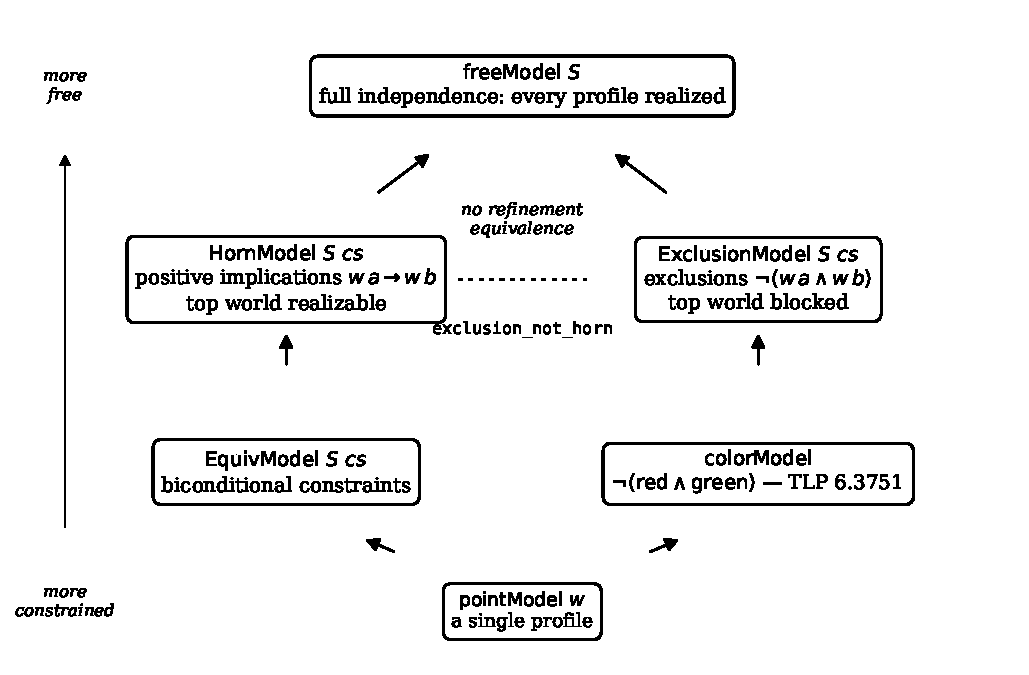
\includegraphics[width=0.82\linewidth]{figures/spectrum.pdf}
  \caption{The world-model spectrum. Arrows are refinements (constraint
  removal); the free model is the maximum (\ref{c:spectrum}). The Horn and
  exclusion tiers are not refinement-equivalent: no Horn model shares a
  nontrivial exclusion model's image profiles
  (Theorem~\ref{thm:exclusion-not-horn}).}
  \label{fig:spectrum}
\end{figure}

\section{World Models and the Free Model}\label{sec:background}

Fix a type $S$ whose elements we read as \emph{states of affairs}
(\emph{Sachverhalte}). The base notions are inherited from the companion
formalization \cite{companion2026}.

\begin{definition}[World model]\label{def:worldmodel}
A \emph{world model} $M$ over $S$ consists of a type $M.W$ of worlds, a
relation $\mathrm{holds}_M : M.W \to S \to \mathrm{Prop}$, and a proof that
$M.W$ is nonempty. The \emph{profile} of a world $w \in M.W$ is the function
$s \mapsto \mathrm{holds}_M(w, s)$, the pattern of states obtaining at $w$.
(Lean: \lean{WorldModel}.)
\end{definition}

\begin{definition}[Free model]\label{def:freemodel}
The \emph{free model} over $S$ takes $\mathit{worlds} = (S \to \mathrm{Prop})$
and $\mathrm{holds}(w, s) = w(s)$: a world just \emph{is} a truth-value
profile, and every profile occurs. (Lean: \lean{freeModel}.)
\end{definition}

The free model is the Tractarian picture of \TLP{1.21} and \TLP{2.062} taken
at face value: any combination of states obtaining and failing is a way the
world could be. Propositions are built from atoms $s \in S$ by negation and
conjunction and evaluated at a world of a model in the obvious way (Lean:
\lean{Proposition}, \lean{evalM}); a proposition is a \emph{tautology of $M$}
when it holds at every $M$-world.

The property that will carry the independence thesis through the paper is:

\begin{definition}[Independent profiles]\label{def:independence}
$M$ \emph{has independent profiles} when every function $S \to \mathrm{Prop}$
is the profile of some $M$-world. (Lean: \lean{HasIndependentProfiles}.)
\end{definition}

This is \TLP{2.062} stated extensionally: nothing about which states obtain
constrains which others do, because every combination is realized. The free
model has independent profiles trivially
(\lean{freeModel\_hasIndependentProfiles}); the question of the paper is what
the landscape looks like when one gives this up.

\section{The Refinement Spectrum}\label{sec:spectrum}

\begin{definition}[Refinement]\label{def:refines}
$M$ \emph{refines into} $M'$, written $M \sqsubseteq M'$, when there is a map
$f : M.W \to M'.W$ with
$\mathrm{holds}_M(w, s) \leftrightarrow \mathrm{holds}_{M'}(f(w), s)$ for all
$w, s$: every $M$-world's profile is realized in $M'$. (Lean: \lean{Refines}.)
\end{definition}

Reading $\sqsubseteq$ upward is \emph{constraint removal}: if
$M \sqsubseteq M'$ then $M'$ realizes at least the ways-the-world-could-be
that $M$ does. The following are elementary but jointly set the stage.

\begin{theorem}[The spectrum]\label{thm:spectrum}
\emph{(i)} $\sqsubseteq$ is reflexive and transitive.
\emph{(ii)} $M \sqsubseteq \mathrm{freeModel}$ for every $M$: the free model
is the maximum of the spectrum.
\emph{(iii)} Evaluation is preserved along refinements: if $f$ witnesses
$M \sqsubseteq M'$ then every proposition has the same truth value at $w$ and
at $f(w)$.
\emph{(iv)} Hence tautologies and contradictions are inherited \emph{downward}:
if $p$ is a tautology (contradiction) of $M'$ and $M \sqsubseteq M'$, then $p$
is a tautology (contradiction) of $M$.
(Lean: \lean{refines\_refl}, \lean{refines\_trans}, \lean{refines\_freeModel},
\lean{refines\_preserves\_eval}, \lean{tautology\_pullback},
\lean{contradiction\_pullback}.)
\end{theorem}

Part (iv) is the formal cash value of the slogan that constraints
\emph{create} necessities: a model lower in the spectrum validates everything
the freer model validates, plus possibly more. The converse direction ---
which propositions are validated \emph{everywhere} --- is answered exactly:

\begin{theorem}[Spectrum-invariant validity]\label{thm:invariant}
A proposition is a tautology of every world model over $S$ iff it is a
tautology of the free model. (Lean:
\lean{spectrum\_invariant\_iff\_freeModel\_tautology}; the forward direction
factors through single-profile \emph{point models},
\lean{pointModel\_isTautology\_iff}.)
\end{theorem}

The logical truths, in this setting, are precisely the propositions
insensitive to the modeling choice. A Tractarian gloss: what holds in
\emph{logic} does not depend on how much independence the world exhibits ---
which is \TLP{6.1}'s ``the propositions of logic are tautologies'' relativized
to the whole spectrum rather than to logical space of the free kind.

Uniqueness gives the free model its privileged status among choices:

\begin{theorem}[Uniqueness of the free model]\label{thm:unique}
If $M$ has independent profiles, then $M$ is refinement-isomorphic to the
free model: there are refinements in both directions. Full independence
determines the model up to the spectrum's own notion of equivalence. (Lean:
\lean{freeModel\_unique\_refines\_iso}.)
\end{theorem}

So the Tractarian choice is well-posed: ``the model on which every
combination of states is possible'' picks out one point of the spectrum. The
substantive question is what lies below it.

\section{The Lattice of Logical Space}\label{sec:lattice}

Refinement, defined via maps of worlds, is captured extensionally by a
simpler invariant.

\begin{definition}[Image profiles]\label{def:image}
$\mathrm{Im}(M) \subseteq (S \to \mathrm{Prop})$ is the set of profiles of
$M$-worlds. (Lean: \lean{ImageProfiles}.)
\end{definition}

\begin{theorem}[Extensionality of refinement]\label{thm:image}
$M \sqsubseteq M'$ iff $\mathrm{Im}(M) \subseteq \mathrm{Im}(M')$; and $M$,
$M'$ are refinement-equivalent (refinements both ways) iff
$\mathrm{Im}(M) = \mathrm{Im}(M')$. Moreover
$\mathrm{Im}(\mathrm{freeModel}) $ is everything. (Lean:
\lean{refines\_iff\_subset\_imageProfiles},
\lean{refinesEquiv\_iff\_image\_eq}, \lean{imageProfiles\_freeModel}.)
\end{theorem}

Up to refinement equivalence, then, a world model over $S$ \emph{is} a
nonempty set of profiles, and the spectrum is the powerset lattice of
$2^S$ minus its bottom. The formalization equips it with the corresponding
operations: a join model realizing the union of two models' profiles, a meet
model realizing the intersection (when nonempty), and an infinitary join,
each characterized by the expected universal property (Lean:
\lean{JoinModel}, \lean{MeetModel}, \lean{iJoinModel} with
\lean{refines\_join\_iff}, \lean{refines\_meet\_iff},
\lean{refines\_iJoin\_iff}).

This is the sense of ``geometry'' in our title, and it earns its keep twice
over. First, it converts questions about world-models-up-to-equivalence into
questions about \emph{which sets of profiles a constraint class can carve
out} --- the form in which the separation theorem of \S\ref{sec:exclusion}
is proved. Second, it locates the Tractarian picture inside a familiar
mathematical object: choosing independence is choosing the top of the
lattice; every alternative model is a region of logical space; and
\TLP{3.42}'s dictum --- that a proposition, though it determines only a
single place in logical space, must already have the whole of logical space
given with it \cite{wittgenstein1921} --- reads naturally as the observation
that the ambient lattice is fixed by $S$ alone, however the modeling choice
restricts the realized region.\footnote{For a recent treatment of logical
form and logical space in the \emph{Tractatus} --- on which places in
logical space reduce to the forms of objects and names --- see Spinney
\cite{spinney2022}; our lattice is a complementary, extensional rendering of
the same geometry, indifferent to what fixes the forms.}

\section{Constraint Tiers: Equivalence, Horn, and the Boundary of
  Independence}\label{sec:tiers}

Arbitrary profile sets are unstructured; the Tractarian dialectic concerns
constraints with an intelligible logical form. Two tiers from the
formalization organize the well-behaved cases.

\begin{definition}[Horn tier]\label{def:horn}
For a list $\mathit{cs}$ of pairs over $S$, the \emph{Horn model}
$\mathrm{Horn}(S, \mathit{cs})$ has as worlds those profiles
$w : S \to \mathrm{Prop}$ satisfying $w(a) \to w(b)$ for every
$(a, b) \in \mathit{cs}$. (Lean: \lean{HornModel}; each pair is a definite
binary Horn clause.)
\end{definition}

\begin{definition}[Equivalence tier]\label{def:equiv}
$\mathrm{Equiv}(S, \mathit{cs})$ has as worlds the profiles satisfying
$w(a) \leftrightarrow w(b)$ for every $(a, b) \in \mathit{cs}$. (Lean:
\lean{EquivModel}.)
\end{definition}

Biconditional constraints are the symmetric closure of implicational ones,
and the formalization makes the containment official: every equivalence model
is refinement-equivalent to the Horn model over the symmetrized clause list,
and refines into the Horn model over the original one (Lean:
\lean{equivModel\_iso\_hornModel\_symm}, \lean{refines\_equivModel\_hornModel}).
Both tiers break independence as soon as they say anything: a clause
$(a, b)$ with $a \neq b$ blocks the profile making $a$ obtain and $b$ fail
(Lean: \lean{hornModel\_independence\_fails},
\lean{equivModel\_independence\_fails}).

What makes the Horn tier more than an example is that its incursion into
independence can be characterized \emph{exactly}.

\begin{theorem}[Exact Horn realizability; the \TLP{2.061} boundary]
\label{thm:horn-boundary}
A Boolean valuation $v : S \to \mathrm{Bool}$ is the profile of some world of
$\mathrm{Horn}(S, \mathit{cs})$ iff $v$ satisfies every clause: for all
$(a, b) \in \mathit{cs}$, if $v(a)$ then $v(b)$. (Lean:
\lean{horn\_valuation\_realizable\_iff}.)
\end{theorem}

The boundary also has a global form, likewise kernel-checked: \emph{every}
profile $S \to \mathrm{Prop}$ is realizable in $\mathrm{Horn}(S, \mathit{cs})$
iff every clause is trivial ($a = b$ for each $(a, b) \in \mathit{cs}$), so
full independence survives a Horn regime exactly when the clause list says
nothing (Lean: \lean{horn\_realizable\_iff}).

Read contrapositively, Theorem~\ref{thm:horn-boundary} says precisely which inferences ``from the
existence of one state of affairs to the existence of another''
(\TLP{2.062}) a Horn regime licenses: exactly the clause-generated ones, and
no others. Independence does not fail catastrophically or holistically; it
fails at the excluded profiles and is retained everywhere else. The
concrete case study in the formalization --- a two-state weather model where
``it rains'' implies ``the street is wet'' --- witnesses the boundary at
minimal scale (Lean: \lean{weatherModel\_equiv\_hornModel},
\lean{weatherModel\_horn\_independence\_fails}).

Theorem~\ref{thm:horn-boundary} is the paper's rendering of what is
\emph{right} in the Tractatus's treatment of constraint: where dependence has
positive-implicational form, logical space contracts in a lawlike,
fully-characterizable way. The next section shows that color exclusion is
not of this form --- provably.

\section{Color Exclusion and the Limits of the Horn Tier}
\label{sec:exclusion}

\TLP{6.3751} locates the mutual exclusion of colors in ``the logical
structure of colour''; the 1929 paper concedes that such exclusions attach to
attributions of degree quite generally and cannot be conjured out of
truth-functional combination \cite{wittgenstein1929}. The formal shape of the
datum is an \emph{exclusion constraint}: two states that cannot both obtain.

\begin{definition}[Exclusion tier]\label{def:exclusion}
$\mathrm{Excl}(S, \mathit{cs})$ has as worlds the profiles satisfying
$\neg(w(a) \wedge w(b))$ for every $(a, b) \in \mathit{cs}$. (Lean:
\lean{ExclusionModel}.)
\end{definition}

The exclusion tier is as well-behaved, taken by itself, as the Horn tier:

\begin{theorem}[Exact exclusion realizability]\label{thm:excl-boundary}
$v : S \to \mathrm{Bool}$ is the profile of some world of
$\mathrm{Excl}(S, \mathit{cs})$ iff no clause $(a, b) \in \mathit{cs}$ has
$v(a)$ and $v(b)$ both true. (Lean: \lean{exclusion\_realizable\_iff}.)
\end{theorem}

\begin{theorem}[Exclusion breaks independence]\label{thm:excl-indep}
If $\mathit{cs}$ is nonempty, $\mathrm{Excl}(S, \mathit{cs})$ does not have
independent profiles --- with no side condition: even a degenerate
self-clause $(a, a)$ forbids $w(a)$ outright, so the all-true profile is
always excluded. (Lean: \lean{exclusionModel\_independence\_fails}; compare
the Horn analog, which needs $a \neq b$.)
\end{theorem}

The asymmetry flagged in Theorem~\ref{thm:excl-indep} is the visible tip of
a structural difference. At the top of every Horn model sits the world where
everything obtains: a positive implication can never rule it out, since its
consequent is true there. Exclusion clauses are defined by ruling it out.

\begin{lemma}[The top world]\label{lem:top}
For every clause list $\mathit{cs}$, the all-true profile lies in
$\mathrm{Im}(\mathrm{Horn}(S, \mathit{cs}))$; for every \emph{nonempty}
$\mathit{cs}$, it does not lie in $\mathrm{Im}(\mathrm{Excl}(S, \mathit{cs}))$.
(Lean: \lean{hornModel\_allTrue\_realizable},
\lean{exclusionModel\_allTrue\_not\_realizable}.)
\end{lemma}

\begin{theorem}[Exclusion is not Horn]\label{thm:exclusion-not-horn}
Let $\mathit{cs}$ be nonempty. There is no clause list $\mathit{ds}$ such
that $\mathrm{Horn}(S, \mathit{ds})$ is refinement-equivalent to
$\mathrm{Excl}(S, \mathit{cs})$. (Lean: \lean{exclusion\_not\_horn}.)
\end{theorem}

\begin{proof}[Proof sketch]
By Theorem~\ref{thm:image}, refinement equivalence is equality of
image-profile sets; by Lemma~\ref{lem:top} the all-true profile separates
any Horn image from any nontrivial exclusion image. The kernel-checked proof
is six lines. \end{proof}

\begin{remark}\label{rem:horn1951}
The top-world lemma is the nullary instance of a classical fact: Horn classes
are closed under intersections of models (in the propositional case,
pointwise conjunction of satisfying assignments), a property isolated by Horn
in 1951 \cite{horn1951} following McKinsey's study of the clause class
\cite{mckinsey1943}. The empty intersection is the all-true assignment.
Exclusion constraints fail closure under intersection in the most flagrant
way available, and Theorem~\ref{thm:exclusion-not-horn} is the Tractarian
payoff of that failure. What our development adds to the classical picture is
the refinement-theoretic phrasing --- no nontrivial exclusion model is
refinement-equivalent to any Horn model, so the tiers are separated in the
model spectrum itself, not merely as distinct syntactic classes --- and the
mechanization.
\end{remark}

The case study instantiates the general theorems at the historically loaded
example. Let $S = \{\mathrm{red}, \mathrm{green}\}$, read as ``point $p$ in
the visual field is red (green)'', and let
$\mathrm{colorModel} = \mathrm{Excl}(S, [(\mathrm{red}, \mathrm{green})])$.

\begin{corollary}[TLP 6.3751, formalized]\label{cor:color}
$\mathrm{colorModel}$ does not have independent profiles, and no Horn
constraint list over $S$ yields a model refinement-equivalent to it. (Lean:
\lean{color\_independence\_fails}, \lean{color\_not\_horn}.)
\end{corollary}

We propose reading Corollary~\ref{cor:color} as a precise statement of what
went wrong in 1929, one that improves on the collapse narrative in two ways.
First, it separates two failures the narrative runs together. That color
exclusion \emph{breaks independence} (the first conjunct) is cheap: any
substantive constraint does that, including the innocuous weather
implication of \S\ref{sec:tiers}. What distinguishes color exclusion is the
second conjunct: it cannot be redescribed within the constraint class whose
incursions into independence are exactly characterizable
(Theorem~\ref{thm:horn-boundary}) and closed under the operations that keep
logical space lawlike. The 1929 crisis was not that the world exhibits
dependence, but that it exhibits dependence of the wrong \emph{shape}.
Second, the reading makes the crisis \emph{stable under reinterpretation}:
Theorem~\ref{thm:exclusion-not-horn} quantifies over all Horn clause lists,
so no rewriting of the color facts in positive-implicational terms can
dissolve it. The theorem does for the color-exclusion problem what
Wittgenstein's own truth-table argument in the 1929 paper gestured at ---
showing the exclusion is not an artifact of notation --- but with the
quantifier over notations made explicit and discharged by the kernel.

\section{Discussion}\label{sec:discussion}

\subsection{Button: cardinality versus structure}

Button proves that the atomist picture tolerates exclusion problems iff
logical space has cardinality a power of two, and reads the result as a
reductio of Tractarian atomism given a continuum of color shades
\cite{button2017}. Our results are complementary but pull in a different
direction: where Button's condition is global and cardinality-theoretic, the
spectrum analysis is local and structural. Theorem~\ref{thm:exclusion-not-horn}
distinguishes exclusion from implication even over a two-element $S$, where
cardinality considerations see nothing (both tiers carve out sets of profiles
of unexceptional sizes). The moral we draw is that ``how big is logical
space?'' undersells the atomist's predicament; the sharper question is
``which regions of the profile lattice can constraints of a given logical
form reach?'' --- and that question has exact answers
(Theorems~\ref{thm:horn-boundary} and \ref{thm:excl-boundary}) that the
cardinality frame cannot express.

\subsection{Moss: re-atomization as a move within the spectrum}

Moss argues the color-incompatibility problem is solvable: choose elementary
propositions wisely (her construction uses vector-valued magnitudes) and the
exclusions come out logical after all \cite{moss2012}. Our framework does not
adjudicate whether her atoms are the right ones; it does clarify what kind of
move she is making. Re-atomization replaces $S$ by a new state-type $S'$ and
relocates the world model: the constrained region of the old lattice is
re-presented as the free top of a new one. Nothing in our theorems obstructs
this --- they are stated for fixed $S$ --- but the spectrum makes the price
explicit: the moves available to the atomist are exhausted by (i) changing
$S$ (Moss), or (ii) descending the lattice for fixed $S$, and
Theorem~\ref{thm:exclusion-not-horn} closes off the hope that descent of a
logically tame (Horn) kind might suffice. The two strategies can then be
evaluated on their merits rather than run together; the formal framework for
comparing atomizations themselves (a map between spectra over different
state-types) is future work, and \S\ref{sec:limitations} records it as such.

\subsection{Combinatorialism}

Armstrong's combinatorial theory of possibility adopts the ``Tractarian
thesis of Independence'' for wholly distinct states of affairs, with
possible worlds as recombinations \cite{armstrong1989}, following Skyrms's
Tractarian nominalism \cite{skyrms1981}. In our terms, combinatorialism is
the decision to model possibility by the free model. The spectrum offers the
combinatorialist a principled fallback under pressure from exclusion
phenomena: rather than defending full recombination or abandoning the
picture, one may occupy a named point lower in the lattice and know exactly
what one has paid --- which recombinations are lost
(Theorems~\ref{thm:horn-boundary}, \ref{thm:excl-boundary}) and which
necessities are gained (Theorem~\ref{thm:spectrum}(iv)). The uniqueness
theorem (\ref{thm:unique}) sharpens the standard observation that
recombination determines the space of worlds: it does so up to exactly the
equivalence the framework itself supplies.

\subsection{Incompatibility as primitive}

Evans and Berger's cathoristic logic takes incompatibility rather than
negation as the primitive logical relation \cite{evans2014}. Their project is
proof-theoretic and ours model-theoretic, but the underlying diagnosis
converges: exclusion is not a derived phenomenon in a logic of positive
combination. Theorem~\ref{thm:exclusion-not-horn} can be read as the
model-theoretic ground for that design decision --- if exclusions were
Horn-expressible, a logic with only positive primitives could simulate them,
and by the theorem it cannot.

\subsection{What the kernel settles}

Every theorem cited above carries a machine-checked proof whose axiom
footprint is \lean{propext}, \lean{Classical.choice}, \lean{Quot.sound} ---
the standard classical base of Lean's mathematical library and nothing else;
no \lean{sorry}s remain. Formal reconstruction of the \emph{Tractatus} is
itself a settled genre --- Lokhorst's axiomatic reconstruction of the
ontology and philosophy of mind \cite{lokhorst1988} and Weiss's systematic
study of the book's logic \cite{weiss2017} are the closest precedents ---
but those reconstructions are checked by hand. We follow the methodological
line of the mechanization of G\"odel's ontological argument
\cite{benzmuller2014}: where a philosophical dispute turns on \emph{what
follows from what}, mechanization relocates the dispute to its honest
residue --- whether the formal explication is faithful. For the present paper that residue is concentrated
in two choices: reading \TLP{2.062}'s independence as
Definition~\ref{def:independence} (realizability of every profile), and
reading color exclusion as a binary exclusion clause
(Definition~\ref{def:exclusion}). Both are defended in situ
(\S\ref{sec:background}, \S\ref{sec:exclusion}); a reader who rejects them
knows exactly where to press, which is the methodological point. In the
interest of full disclosure required by the method: statements and proofs of
the exclusion-tier module, and the per-valuation Horn boundary lemma of
Theorem~\ref{thm:horn-boundary}, were developed with an AI assistant and
verified by the Lean kernel; the spectrum, Horn, and equivalence modules
originate in the companion project \cite{companion2026}, with
machine-verified proofs throughout (see Acknowledgments).

\section{Limitations}\label{sec:limitations}

\emph{States of affairs are unstructured.} $S$ is a bare type: states have
no inner composition of objects, so the account cannot yet express
\emph{why} red and green exclude (their sharing a determinable), only
\emph{that} an exclusion constraint is in force. A dependent-type treatment
of objects, making independence claims sensitive to constituent-sharing, is
the natural continuation (and was flagged as future work in the companion
paper).

\emph{Binary clauses.} Both the Horn and exclusion tiers use binary clause
lists. $n$-ary Horn clauses and pairwise-exclusion families (a determinable
with $k$ determinates, e.g.\ a full color space) are unproblematic
extensions of the definitions, but the theorems above are proved for the
binary case; we expect Theorem~\ref{thm:exclusion-not-horn}'s top-world
argument to lift without incident, since it uses only the nullary closure
instance.

\emph{Fixed atomization.} The spectrum is indexed by a fixed $S$; comparing
models across state-types --- needed to fully engage Moss's re-atomization
strategy --- requires a notion of spectrum morphism we have not developed.

\emph{Explication risk.} The kernel checks proofs, not faithfulness. Our
\TLP{2.061}/\TLP{2.062} and \TLP{6.3751} readings are argued for but not
beyond dispute; in particular, readers who take Tractarian elementary
propositions to be constitutively independent (so that ``constrained
elementary propositions'' is a contradiction in terms) will read the spectrum
as charting successors to the Tractarian picture rather than variants of it.
The theorems are indifferent to this choice of description.

\emph{No degree structure.} The 1929 paper's own diagnosis involves
attributions of degree and the joint syntax--phenomenology of measurement.
Our exclusion clauses capture the resulting incompatibilities extensionally
but say nothing about degrees as such.

\section{Conclusion}\label{sec:conclusion}

Treating the Tractatus's independence thesis as a modeling choice replaces a
binary dispute --- independence: true or refuted? --- with a structured
space of positions, and the structure turns out to be theorem-rich. The free
model sits at the top of a refinement lattice whose geometry is exactly the
powerset of profiles; spectrum-invariant validity coincides with free-model
tautology; full independence determines the model uniquely up to the
lattice's own equivalence. Constraint classes occupy the lattice as tiers
with exactly characterizable reach, and the constraint that historically
broke the book --- color exclusion --- provably outruns the reach of the
positive-implicational tier. On this telling, the color-exclusion problem
was never a mere counterexample awaiting a clever re-atomization or a
regretful abandonment; it was the discovery, made without the benefit of the
lattice in which to state it, that logical space has regions of essentially
different shape. The machine-checked development makes that discovery a
theorem, and the spectrum gives both the Tractarian and her critics named
positions to occupy --- with prices marked.

\subsubsection*{Acknowledgments}

The base formalization of worlds, propositions, and evaluation, together with
the spectrum, Horn-tier, and equivalence-tier modules, was developed in the
companion project \cite{companion2026}; several of the ported modules'
theorems were proved by Harmonic's Aristotle system from our statements, as
acknowledged there. The exclusion-tier module (statements and proofs) and
the per-valuation Horn realizability lemma
(\lean{horn\_valuation\_realizable\_iff}) were
developed with Claude (Anthropic) in the course of preparing this paper. All
proofs, whatever their origin, are checked by the Lean~4 kernel; the axiom
footprint of every theorem cited here is \lean{propext},
\lean{Classical.choice}, \lean{Quot.sound} only.

\appendix

\section{Theorem Index}\label{app:index}

All declarations reside in the four modules
\begin{center}
\lean{proofs/TractatusOntology\{Horn,\,Equiv,\,Spectrum,\,Exclusion\}.lean}
\end{center}
of the \lean{tractatus} repository,
\url{https://github.com/rjwalters/tractatus}; the build is warning-free
under Lean~4.26 with no \lean{sorry}s.

\begin{center}
\small
\begin{tabular}{@{}lll@{}}
\toprule
Paper & Lean declaration & Module \\
\midrule
Thm~\ref{thm:spectrum}(i) & \lean{refines\_refl}, \lean{refines\_trans} & Spectrum \\
Thm~\ref{thm:spectrum}(ii) & \lean{refines\_freeModel} & Spectrum \\
Thm~\ref{thm:spectrum}(iii) & \lean{refines\_preserves\_eval} & Spectrum \\
Thm~\ref{thm:spectrum}(iv) & \lean{tautology\_pullback}, \lean{contradiction\_pullback} & Spectrum \\
Thm~\ref{thm:invariant} & \lean{spectrum\_invariant\_iff\_freeModel\_tautology} & Spectrum \\
Thm~\ref{thm:unique} & \lean{freeModel\_unique\_refines\_iso} & Spectrum \\
Thm~\ref{thm:image} & \lean{refines\_iff\_subset\_imageProfiles}, \lean{refinesEquiv\_iff\_image\_eq} & Spectrum \\
(lattice ops) & \lean{JoinModel}, \lean{MeetModel}, \lean{iJoinModel} + characterizations & Spectrum \\
Thm~\ref{thm:horn-boundary} & \lean{horn\_valuation\_realizable\_iff} & Horn \\
(global Horn boundary) & \lean{horn\_realizable\_iff} & Horn \\
(Horn indep.\ fails) & \lean{hornModel\_independence\_fails} & Horn \\
(Equiv $\to$ Horn) & \lean{equivModel\_iso\_hornModel\_symm}, \lean{refines\_equivModel\_hornModel} & Equiv \\
Thm~\ref{thm:excl-boundary} & \lean{exclusion\_realizable\_iff} & Exclusion \\
Thm~\ref{thm:excl-indep} & \lean{exclusionModel\_independence\_fails} & Exclusion \\
Lem~\ref{lem:top} & \lean{hornModel\_allTrue\_realizable}, & Exclusion \\
 & \lean{exclusionModel\_allTrue\_not\_realizable} & \\
Thm~\ref{thm:exclusion-not-horn} & \lean{exclusion\_not\_horn} & Exclusion \\
Cor~\ref{cor:color} & \lean{color\_independence\_fails}, \lean{color\_not\_horn} & Exclusion \\
\bottomrule
\end{tabular}
\end{center}

\bibliographystyle{plain}
\bibliography{refs}

\end{document}
